\section{\sys Design} \label{xsnare_design}

 \begin{figure}[h]
	\includegraphics[scale=0.55]{img/xsnare.pdf}
	\caption{\sys's approach to protect against XSS.}
	\label{fig:xsnare}
\end{figure}

We now present the design of \sys and its components. % and how they interact with each other.
%
% \subsection{Operation, at a glance} \label{operation}
%
We begin with a high-level view of its operation (see
\autoref{fig:xsnare}): A user requests a page, \url{example.com}, on a
browser with the \sys extension installed.
%
The response may or may not contain
malicious \xss payloads.
%
Before the browser renders the document, \sys analyzes
the potentially malicious document. The extension loads signatures
from its local database into its detector. The detector analyzes the
HTML string arriving from the network, and identifies the signatures
which apply to the document. These signatures specify one or more
``injection spots'' in the document, which correspond, roughly
speaking, to regions of the DOM where improperly sanitized content
could be injected.  The extension's sanitizer
eliminates any malicious content and outputs a clean HTML document to
the browser for rendering (\autoref{filter_algorithm}).

%% The network filter is presented in \autoref{filter_algorithm} describes the
%% network filtering process. Section \ref{implementation} explains this
%% algorithm in more detail.

\subsection{An example application of \sys} \label{motivating_example}

To further explain our approach, we present a small example of how
DOM context can be used to defend against XSS, taken from CVE
2018-10309~\cite{examplecve}. This is reproducible in an off-the-shelf
WordPress installation running the Responsive Cookie Consent plugin,
v1.7. This is a stored \xss vulnerability, and as such is not caught
by some generic client-side \xss filters, including Chrome's XSS auditor.

Consider a website running PHP on the backend which stores user input
from one user, and displays it later to another user, inside an \textbf{input} element.

The PHP code defines the static HTML template (in black), as well as the dynamic input (in red):

\begin{lstlisting}
<input id="rcc_settings[border-size]" 
name="rcc-settings[border-size]" 
type="text" value=<@\textcolor{red}{"<?php rcc\_value('border-size'); ?>"}@>/>
<label class="description"
for="rcc_settings[border-size]">
\end{lstlisting}
Under normal circumstances, the \textbf{input} might have a value of "0":
\begin{lstlisting}
<input id="rcc_settings[border-size]" 
 name="rcc-settings[border-size]" 
 type="text" value=<@\textcolor{red}{"0"}@>>
<label class="description"
 for="rcc_settings[border-size]">
\end{lstlisting}
However, the php code is vulnerable to an injection attack, e.g.:
\begin{lstlisting}
border-size = ""><script>alert('XSS')</script>
\end{lstlisting}
The browser will render this, executing the injected script:
\begin{lstlisting}
<input id="rcc_settings[border-size]" 
name="rcc-settings[border-size]" 
type="text" value=<@\textcolor{red}{""><script>alert('XSS')</script>}@>
<label class="description"
for="rcc_settings[border-size]">
\end{lstlisting}

Note that the resulting HTML is well-formed, so a mere syntactic check
will not detect the malicious injection. Let us assume a security
analyst knows the original template, i.e., without injected
content. If the analyst were given a filled-in document, they could
(in most cases) separate the injected content from the server-side
template, and get rid of the malicious script entirely, using proper sanitization. %\sys essentially automates the decision and sanitization process.

The injected script is bounded by template elements with identifiable
attributes. Assuming (for now) that there is only one such vulnerable
injection point, we can search for the \textbf{input} element from the
top of the document, and the \textbf{label} from the bottom to ensnare
the injection points in the HTML.

This shares goals with the client/server hybrid approach of Nadji et
al.~\cite{Nadji:2009}. They automatically tag injected DOM elements on the
server-side using a taint-tracking, so that the client (a
modified browser) can reliably separate template vs
injected content. We do not require any server-side modifications, but rather opt for a client-side tagging solution based on exploit definitions.

The injected content, once identified, must be sanitized appropriately.
The appropriate action will depend on the application setting, but
assuming a patch has been written, it suffices to translate the
intention in the server code's path to the client-side.
This can be straightforward, once the fix is understood.
%but the application developer's intention might not always be clear.

The developer incorrectly claimed the bug had
been fixed in version 1.8 of the plugin.
Other similar vulnerabilities had indeed been fixed, but not this one~\cite{rccpatch}. The built-in WordPress function \code{sanitize\_text\_field} needed to be applied.
%%which sanitizes the parameters by
%%checking for common invalid characters like invalid UTF-8.

\xss does not automatically determine the relevant actions to
implement from a patch. We assign this task to a security
analyst, who will act as the signature developer for a given
exploit. The system will however automate the signature matching and
sanitization.

%% In the following sections we give a detailed description of each
%% component of our system, the challenges that arise when trying to
%% defend against XSS client-side, and the tools provided by the browser
%% to facilitate our methods.

\subsection{\sys Signatures} \label{signatures}

%The signatures are at the core of XSnare.

%% this is a repeat with the next section
%% Signatures rely heavily on document structure. They must be
%% conservative enough to capture all of the injected content, yet be
%% precise enough to affect only specific elements of specific pages.
%% %
%% %
%Since we are only relying on DOM knowledge,
%% These signatures rely heavily HTML features, for example,
%% specifying elements and attributes that are unique to where the
%% exploit might occur.


Our signature definitions make two assumptions: first,
\textbf{an injection must have a start point and end point}, that is,
an element can only be injected between a specific HTML node and its
immediate sibling in the DOM tree; second, in a well-formed DOM,
\textbf{the dynamic content will not be able to rearrange its location
  in the document without JavaScript execution} (e.g., removing and
adding elements), allowing us to isolate it from the template.

Pages commonly contain more than one vulnerable injection point.
We discuss the difficulty of supporting these pages in \autoref{multiple_injections}.

We believe CVEs are an ideal growing source of signature
definitions. Since previous client-side work does not focus on
application-specific protection, these tools often use less accurate
heuristics to detecting exploits. Furthermore, once new
vulnerabilities are found, these systems often lack the
maintainability obtained by leveraging active CVE development.
%Our system assumes signatures are written by a third-party:
%% Pentesters will commonly identify
%% new issues with application code, inform developers and publish them for the
%% benefit of the community in the form of CVEs.

We are conscious that \sys signatures will not write themselves, and that
this task represents a new step in the workflow. Luckily, converting
the CVE information into a signature does not require active
participation from the application developers -- Security enthusiasts and
web developers have the skills to fulfill this role satisfactorily.

Long term, we imagine that volunteers (or entrepreneurs) would
cultivate and maintain the signature database. New signatures could be
contributed by a community of amateur or professional security analysts, in a manner not
so different from how antispam or antivirus software is managed.
% We don't perceive this development model to be radically different from existing ones.

The challenge of automatically deriving signatures from detailed CVEs is an interesting
one, albeit outside the scope of this paper.

%Thus, the signature database is maintained by a trusted entity which
%audits CVEs, and a malicious analyst cannot take advantage of this
%model to harm the user's browsers through signatures. An analyst can
%write a signature in our language given their knowledge of the
%exploit, as they will often know both the source and the way it
%manifests in the HTML, as well as the fix.

 \subsection{Firewall Signature Language} \label{signature_language}

 Our signature language needs to be such that it has enough power of
 expression for the signature writer to be precise, both for
 determining the correct web application and to identify the affected
 areas in the HTML. For injection point isolation, a language based on
 regular expressions suffices to express precise
 sections of the HTML. The following is the signature that defends
 against the motivating example of \autoref{motivating_example}:

 \begin{lstlisting}[breaklines=true,caption={An \sys signature},label={lst:xsnare_signature}]
url: 'wp-admin/options-general.php?page=rcc-settings',
software: 'WordPress',
softwareDetails: 'responsive-cookie-consent',
version: '1.5',
type: 'string',
typeDet: 'single',
sanitizer: 'regex',
config: '/^[0-9](\.[0-9]+)?$/',
endPoints: 
['<input id="rcc_settings[border-size]" name="rcc_settings[border-size]" type="text"
  value="',
'<label class="description" 
for="rcc_settings[border-size]">']
\end{lstlisting}

A description of the development process for this signature is given
in Section \ref{case_study}. In summary, a signature will have the
necessary information to determine whether a loaded page has a
vulnerability, and specify appropriate actions for eliminating
any malicious payloads.

%% Once the page's identifying information and the dynamic content is
%% established by an analyst,
Analysts configure their signatures with one
function chosen from the static set of sanitization
functions offered by \sys. These functions inoculate potentially malicious injections
based on the DOM context surrounding the injection. The goal of
signatures is to provide such sanitization, ideally without ``breaking''
the user experience of the page. The default function preset is DOMPurify's~\cite{10.1007/978-3-319-66399-9_7} default
configuration,
%% \footnote{This library is described by its creators as a
%%   "DOM-only, super-fast, uber-tolerant XSS sanitizer for HTML, MathML
%%   and SVG". The Mozilla community cites it as an useful tool for
%%   "safely inserting external content into a
%%   page"~\cite{safecontent}}
which takes care of common sanitization needs~\cite{safecontent}. However, DOMPurify's defaults can be unnecessarily restrictive, in which cases the other sanitization methods are more desirable.

We considered allowing arbitrary sanitization code in
signatures. While it would open complex sanitization possibilities, we
have decided against it, principally for security reasons. The minimal
set of functions we settled on also sufficed to express all of the
signatures defined for this paper.

%% \begin{enumerate} 
%% 	\item Security Concerns: We assume signatures come from a trusted source. However, partly due to the way they are currently stored, it is possible for an attacker to add malicious signatures. In general, this would only harming the web site user experience by removing safe content. The ability to run arbitrary code would lead a serious security flaw, as it would execute in a high-privilege environment.
%% 	\item Case Coverage: While our provided methods might be limited in some scenarios, we have applied them in our studied CVEs with positive results, and are confident they can cover most use cases.
%% 	\item Adoption: A declarative language will help signature developers expedite the process of writing signatures, as they will find that our provided methods will most often suffice.
%% \end{enumerate}

 \subsection{Firefox Extension} \label{firefox_extension}

 Our system's main component is a browser extension which rewrites
 potentially infected HTML into a clean document.
 %% % this is a repeat
 %% We believe an
 %% extension to be ideal for our purposes due to the context available
 %% to it.
 %% Previous client-side work has focused on browser modifications
 %% and higher-level tools. These tools do not have the context required
 %% for the application-specific behaviour we seek.  The extension
 detects exploits in the HTML by using signature definitions and
 maintains a local database of signatures. We leave the design of an
 update mechanism to future work, but in its current form, the
 database is bundled with each new installation of the extension.
 %

 The extension translates signature definitions into patches that
 rewrite incoming HTML on a per-URL basis, according to the top-down,
 bottom-up scan described in \autoref{motivating_example}.
 
 The extension's detector acts as an in-network filter. We initially considered other designs but quickly found out that applying the patch at the network level was necessary for sanitization correctness: even before any code runs, parsing the HTML into a DOM tree
might cause elements to be re-arranged into an unexpected order,
making our extension sanitize the wrong spot.  Consider the following
example, where an element inside a <tr> tag is rearranged after
parsing the string:

\begin{lstlisting}
<table class="wp-list-table">
  <thead>
     <tr>
	     <th></th>
	     <@\textcolor{red}{<img src="1" onerror="alert(1)">}@>
	     <th>
   	     <form method="GET" action="">
...
\end{lstlisting}

In this HTML, the signature developer might identify the exploit as
occurring inside the given table. However, if we wait until the string
has been parsed into a DOM tree to sanitize, the elements are
rearranged due to <tr> not allowing an <img> as its child:

\begin{lstlisting}
<@\textcolor{red}{<img src="1" onerror="alert(1)">}@>
<table class="wp-list-table">
   <thead>
   <tr>
	   <th></th>
	   <th>
       <form method="GET" action="">
...
\end{lstlisting}

Note that the injected <img> tag is now outside of the table, simply
by virtue of the DOM parsing. Now, the extension will search past the
injection, as it occurs before the table element, creating a false
negative (FN). Similarly, elements rearranged inside an injection
point can create false positives. This example would generate a class
of circumvention techniques for our detector, so we can't wait until
the website has been rendered to analyze the response. This guarantees
that a knowledgeable attacker can not take advantage of this
behavior.

\subsection{Handling multiple injections in one page} \label{multiple_injections}

In Listing \ref{lst:xsnare_signature}, the endPoints were listed as
two strings in the incoming network response. However, there are cases
where arbitrarily many injection points can be generated by the
application code, such as a for loop generating table rows. For these,
it is hard to correctly isolate each endPoint pair, as an attacker
could easily inject fake endPoints in between the original ones.

\begin{figure}[h]
	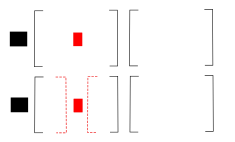
\includegraphics[scale=0.25]{img/attacker_injection_compound.pdf}
	\caption{Example attacker injection when multiple injection points exist in the page. a) a basic injection pattern. b) an attempt to fool the detector.}
	\label{fig:attacker_injection}
\end{figure}

In Figure~\ref{fig:attacker_injection}a, the brackets indicate a
template. The content in between is an injection point (the star),
where dynamic content is injected into the template. In the case of a
vulnerability, the injected content can expand to any arbitrary
string. The signature separates the injection from the rest by
matching for the start and end points (the \code{endPoints}),
represented by the brackets. This HTML originally has two pairs of
\code{endPoint} patterns.

In Figure~\ref{fig:attacker_injection}b, the attacker knows these are
being used as injection end points and decides to inject a fake ending
point and a fake starting point (the dotted brackets), with some
additional malicious content in between. If just looking for multiple
pairs of end points, the detector cannot tell the difference between
the solid and dotted patterns, and will not get rid of the content
injected in the star. Therefore, we have to use the first starting
point and the last ending point before a starting one (when searching
from the bottom-up) and sanitize everything in between. This might get
rid of a substantial amount of valid HTML, so we defer to the
signature developer's judgment of what behavior the detector should
follow. We expand upon this further in \autoref{case_study}.


\begin{figure}[h]
	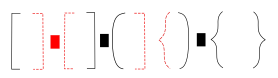
\includegraphics[scale=0.25]{img/attacker_injection_unique.pdf}
	\caption{Example attacker injection when multiple distinct injection points exist in the page.}
	\label{fig:attacker_injection_unique}
\end{figure}


Figure ~\ref{fig:attacker_injection_unique} illustrates a case when
there are several injection points in one page, but each of them is
distinct. Now, the filter is only looking for one pair of brackets, so
the attacker can't fool the extension into leaving part of the
injection unsanitized. However, they could, for example, inject an
extra ending bracket after the opening parenthesis (or an extra
starting brace). The extension will be tricked into sanitizing
non-malicious content, the black pluses (+). This behavior can be
detected by noting that we know the order in which the
\code{endPoints} should appear, and so if the filter sees a closing
\code{endPoint} before the next expected starting \code{endPoint}, or
similarly, a starting \code{endPoint} before the next expected closing
\code{endPoint}, this attack can be identified. In the diagram, the
order of the solid elements characterizes the possible malformations
in the end points. As with the previous scenario, we have to sanitize
the outermost end points, potentially deleting non-malicious
content. The signature developer specifies the sanitization behavior.

\subsection{Dynamic injections} \label{dynamic_injections}

The top-level documents of web pages fetch additional dynamic content
via \js{fetch} or AJAX APIs. Content fetched in
this way is also vulnerable to \xss, and must be filtered. An example
vulnerability is CVE-2018-7747 (WordPress Caldera Forms, which allows malicious
content retrieved from the plugin's database to be injected in response to a click.

\sys allows XHR requests to be filtered with \js{xhr}-type
signatures. To reduce the number of signatures that need to be
considered when a browser issues a request, we require that signatures
for XHR be nested inside a signature for a top-level document. If a
page's main content matches an existing top-level signature description,
\sys will then enable all nested XHR listeners.

Signatures for dynamic requests are specified in the \js{listenerData}
key, which includes a listener type and method. The idea is extensible
to scripts and other objects loaded separately from the main document
(e.g., images, stylesheets, etc.).

\begin{lstlisting}[breaklines=true,caption={
      An example dynamic request signature. This patches CVE-2018-7747.
    },label={lst:dynamic_signature}]
...
listenerData: [{
  listenerType: 'xhr', listenerMethod: 'POST',
  sanitizer: 'escape', type: 'string',
  listenerUrl: 'wp-admin/admin-ajax.php',
  typeDet: 'single-unique',
  endPoints: ['<p><strong>', '[AltBody]']
}]
\end{lstlisting}

